
\begin{problem}

Read Section 15.1 (pages 368--376) of\emph{The Pleasures of Counting}
by Koerner (posted on Canvas) and do Exercises 15.1.1--15.1.3.
\end{problem}

\noindent
\includegraphics[width=150mm]{15.1.1}

\includegraphics[width=150mm]{15.1.2}

\newpage
\begin{Answer}

\begin{enumerate}
  \item 15.11

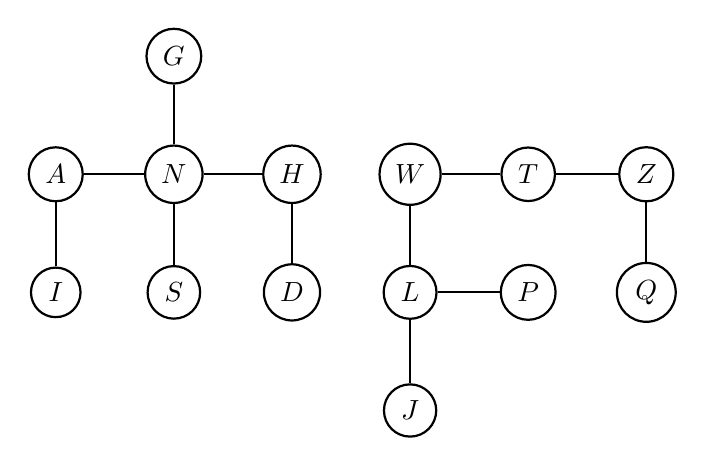
\begin{tikzpicture}[node distance={15mm}, thick, main/.style = {draw, circle}] 
\node[main] (A) {$A$}; 
\node[main] (N) [right of=A] {$N$}; 
\node[main] (H) [right of=N] {$H$}; 
\node[main] (G) [above of=N] {$G$}; 
\node[main] (I) [below of=A] {$I$};
\node[main] (S) [below of=N] {$S$};
\node[main] (D) [below of=H] {$D$};

\node[main] (W) [right of=H] {$W$}; 
\node[main] (T) [right of=W] {$T$}; 
\node[main] (Z) [right of=T] {$Z$}; 
\node[main] (L) [below of=W] {$L$}; 
\node[main] (P) [below of=T] {$P$};
\node[main] (Q) [below of=Z] {$Q$};
\node[main] (J) [below of=L] {$J$};

\draw (A) -- (N);
\draw (N) -- (H);
\draw (N) -- (G);
\draw (A) -- (I);
\draw (N) -- (S);
\draw (H) -- (D);

\draw (W) -- (T);
\draw (T) -- (Z);
\draw (Z) -- (Q);
\draw (W) -- (L);
\draw (L) -- (P);
\draw (L) -- (J);

\end{tikzpicture}

\item 15.12


\item{15.13}
\end{enumerate} 
\end{Answer}
